\documentclass[11pt]{extarticle}
\usepackage{manualdoprofessor}
\usepackage{fichatecnica}
\usepackage{lipsum,media9}
\usepackage[justification=raggedright]{caption}
\usepackage[one]{bncc}
\usepackage[werner]{../edlab}
\usepackage{marginnote}
\usepackage{pdfpages}
\usepackage[printwatermark]{xwatermark}
\newwatermark[pagex=2]{
\includegraphics[scale=3.3]{watermarks/test-a.png}}	% página específica
%\newwatermark[oddpages]{
\includegraphics{watermarks/test-a.png}}			% páginas ímpars
%\newwatermark[evenpages]{
\includegraphics{watermarks/test-a.png}}			% págimas pares
\newwatermark[allpages]{
\includegraphics[scale=3.3]{watermarks/test-b.png}}

\pagecolor{cyan!0!magenta!10!yellow!28!black!28!}

\newcommand{\AutorLivro}{Camila Werner}
\newcommand{\TituloLivro}{Bom dia, Calu}
\newcommand{\Tema}{Quotidiano de crianças nas escolas; nas famílias e nas comunidades (urbanas e rurais)}
\newcommand{\Genero}{Narrativos: fábulas originais; da literatura universal e da tradição popular; etc}
%\newcommand{\imagemCapa}{./images/PNLD0001-01.png}
\newcommand{\issnppub}{978-65-99583-61-2}
\newcommand{\issnepub}{978-65-99583-63-6}
% \newcommand{\fichacatalografica}{PNLD0001-00.png}
\newcommand{\colaborador}{{Paulo Pompermaier e Renier Silva}}

\begin{document}

\title{\TituloLivro}
\author{\AutorLivro}
\def\authornotes{\colaborador}

\date{}
\maketitle

%\begin{abstract}\addcontentsline{toc}{section}{Carta ao professor}
%\pagebreak

\tableofcontents



\section{Sobre o livro}

%550 caracteres
\paragraph{O livro} \textit{Bom dia, Calu}, de Camila Werner, apresenta as diversas possibilidades e escolhas com as quais nos deparamos no dia a dia. 
Desde que levanta da cama, a protagonista Calu encontra várias escolhas
a tomar: a roupa que vai vestir, o que comer no café da manha e no almoço,
como ir para a escola, do que brincar. As ilustrações, de Manuella Silveira, complementam a história ao trazer, para o campo visual, as diferentes opções disponíveis para Calu.
Com tantas escolhas, cada dia se faz único, e valorizamos desde pequeno o ato de escolher.


%822 caracteres
\paragraph{Descrição} O livro percorre os diversos momentos do dia de Calu: quando acorda, veste-se, toma o café da manhã, vai para a escola, escuta histórias e canta músicas com os colegas, brinca no recreio, até retornar a casa para almoçar, tirar a soneca da tarde e se banhar para a hora de dormir. As frases curtas, narrando esses momentos, são acompanhadas por ilustrações nos dois lados de cada dupla de páginas.
Dispostas assim, as imagens evidenciam as diferentes opções para cada momento, ou os diferentes elementos que fazem parte de cada atividade. O acordar, por exemplo, é ilustrado pelo sol, de um lado, e do outro a cama. Para se vestir há duas opções: um vestido ou camiseta e shorts. Igualmente, na hora de lanchar, pode escolher uma fruta ou uma bolacha, sempre representadas lado a lado. Os textos sugerem que é preciso fazer uma escolha, mas não indicam qual dos elementos foi escolhido ou é da preferência da personagem. ``No café da manhã, Calu gosta de comer\ldots'', podemos ler em um dos trechos. Cabe ao leitor, portanto, completar a resposta, escolhendo entre uma das ilustrações apresentadas ou escolhendo outros elementos de sua imaginação e sua experiência pessoal.

%411 caracteres
\paragraph{Competências}
O livro \textit{Bom dia, Calu}, pela forma como é composto, permite trabalhar e explorar diversas competências com as crianças. O próprio enredo da história já traz uma habilidade fundamental a ser desenvolvida com a criança: a capacidade de tomar uma decisão consciente. E isso é feito apenas com elementos e ações do cotidiano da criança, trazendo ao seu universo a história e, assim, ampliando seu enredamento na narrativa. Como o livro convida o leitor a interagir com o livro, apresentando duas opções para cada escolha da protagonista, também é uma ótima forma de trabalhar a criatividade e imaginação dos alunos, convidando-os a ter um papel ativo na narração.


%862 caracteres
\paragraph{Aprofundamento} Este material tem a 
intenção de contribuir para que você consiga desenvolver um trabalho aprofundado 
com esta obra na sala de aula. Você encontrará informações sobre a autora, sobre 
o gênero e sobre os temas trabalhados ao longo do livro. Apresentaremos também 
algumas propostas de trabalho para a sala de aula que você poderá explorar livremente, 
da forma que considerar mais apropriada para os seus estudantes. Para a prática 
da Literacia Familiar, oferecemos um guia que pode ajudar nas orientações aos 
responsáveis pela criança, para incentivar o gosto pela leitura e contribuir para 
que os estudantes desenvolvam em casa habilidades que serão importantes no momento 
da alfabetização. Por fim, você encontrará sugestões de livros, artigos e sites 
selecionados para enriquecer a sua experiência de leitura e, 
consequentemente, a de seus estudantes.



\section{Sobre os autores}

%532 caracteres
\paragraph{O autor} 

%313 caracteres
\paragraph{Publicações}

%358 caracteres
\paragraph{Currículo} 


\section{Sobre o gênero}

%55 caracteres
\paragraph{O gênero} O gênero deste livro é \textit{narrativa}. 

%596 caracteres
\paragraph{Descrição} Em sua base, pode-se definir a narrativa como um gênero que conta uma história, normalmente em estrutura linear, ou seja, começo, meio e fim, e com personagens. 
Dentre os tipos de narrativas mais comuns na literatura infantil, estão: mito, lenda, 
fábula e apólogo. Nos livros infantis, as possibilidades narrativas são quase ilimitadas, pois quase tudo pode integrar a narrativa e fazer parte dela como personagem, já que a capacidade reflexiva das crianças nesta idade ainda está em um nível primário. 



%603 caracteres
\paragraph{Interação} As narrativas são uma forma de inserir os sujeitos no mundo. 
São elas que apresentam boa parte dos valores culturais da sociedade 
onde se vive. Mas não é só passivo o papel das crianças nesta experiência. 
As interações entre dois ou mais personagens onde se verifica
uma ação de linguagem organiza e impulsiona experiências compartilhadas,
importantes para o desenvolvimento psíquico do sujeito nos primeiros anos de vida.
Neste sentido, as narrativas são uma ótima ferramenta para
apresentar o mundo e capacitar as crianças para viver nele, mas como se
trata de um trabalho com a linguagem, sempre dando espaço à individualidade, 
seja na compreensão das histórias, na identificação com as personagens, ou 
no ato de narrar.

%862 caracteres
\paragraph{Competências} 
Através de elementos dos mitos, contos e histórias do cotidiano (como é o caso desse livro), desenvolve-se a sensibilidade narrativa e a capacidade de imaginação das crianças. Para um bom desenvolvimento da capacidade narrativa e imaginativa é necessária a intermediação do educador, que vai trazer novos olhares, análises e discussões para ajudar a criança na construção do significado. Essas são etapas fundamentais para o desenvolvimento linguístico e a aquisição das competências de leitura e escrita. Por meio da narrativa, inclusive, a criança passa do diálogo ao monólogo, pois passa a ser capaz de elaborar um discurso para si com maior autonomia, sem a intermediação necessária no diálogo.
O conjunto de elementos verbais e visuais da narrativa proporcionam, assim,
uma abertura ao mundo e um convite para integrá-lo pela curiosidade e pela imaginação.


\section{Temas}

\subsection{Quotidiano de crianças nas escolas; nas famílias e nas comunidades (urbanas e rurais)}

%136 caracteres
\paragraph{Abordagem} Toda a narração centra-se no quotidiano de uma criança, trazendo atividades típicas da experiência social dos alunos: acordar, ir para a escola, ouvir histórias na sala de aula, almoçar, brincar com os colegas, dormir etc.

%206 caracteres
\paragraph{Descrição} O livro oferece uma ótima oportunidade de explorar 
e aprofundar a relação da criança com a sociedade, trabalhando as escolhas que devemos fazer no dia a dia e relacionando-as a experiências comuns do quotidiano de uma criança pequena. Ao convidar o leitor a interagir diretamente com as decisões de Calu, também estimula a imaginação e a identificação com a história narrada.

%275 caracteres
\paragraph{Competências} Este tema relaciona-se, principalmente, ao 
campo da experiência O eu, o outro e o nós 
descrito pela \textsc{bncc}, que explora as relações interpessoais das crianças e sua capacidade de criar vínculos, percebendo os diálogos e escolhas que constituem a vida em sociedade.


\section{Modelagem de aula}
A seguir você encontrará a descrição de uma aula modelo como exemplo 
prático de exploração do livro com estudantes. Esta seção apresentará 
orientações sobre como organizar a sala de aula para receber os 
estudantes, exercitar a interação verbal e prepará-los para o 
momento da leitura.

Em seguida, você encontrará a \textbf{Leitura dialogada}, um 
tópico destinado a te orientar para o momento específico da 
leitura com os estudantes. Por fim, no tópico 
\textbf{Propostas de atividades}, você encontrará ideias 
de práticas que pode explorar com as crianças em sala de 
aula antes, após e durante a leitura. 

Essas atividades podem ser trabalhadas de acordo com a 
disponibilidade do seu cronograma. Fique à vontade para adaptá-las 
da forma que achar melhor para os seus estudantes. Cada turma é única 
e o seu conhecimento prático das características de cada aluno será 
essencial para definir a melhor forma de aplicar essas ideias. 

O objetivo deste manual é oferecer algumas ideias 
e inspirações para um trabalho que pode ser desenvolvido tanto 
a curto, quanto a médio e longo prazo. Sinta-se à vontade para 
personalizar a aula e torná-la sua, aplicando seus conhecimentos, sua 
personalidade e aproveite para fortalecer 
seu vínculo com a turma.


\subsection{Antes de ler}

\BNCC{EI02EO01}
\BNCC{EI02EO02}
\BNCC{EI02EO03}
\BNCC{EI02EO04}
\BNCC{EI02EO06}
\BNCC{EI02EO07}
\BNCC{EI02EF01}
\BNCC{EI02ET06}

%Alterar o nível escolar nesse parágrafo.
Como este trabalho será realizado com crianças da \textbf{Creche 2}, 
que ainda não têm tanta intimidade com o livro enquanto objeto, você terá o 
papel essencial de mediar este contato. 

Nosso objetivo é que os próprios estudantes possam manusear 
e explorar o livro de forma autônoma, mas, para que isto aconteça, você 
pode ajudar a tornar o caminho mais convidativo com atividades que tenham 
intencionalidade educativa. 

A \textsc{bncc} define intencionalidade educativa como ``organização 
e proposição, pelo educador, de experiências que permitam às crianças 
conhecer a si e ao outro e de conhecer e compreender as relações com a 
natureza, com a cultura e com a produção científica, que se traduzem nas 
práticas de cuidados pessoais (alimentar-se, vestir-se, higienizar-se), 
nas brincadeiras, nas experimentações com materiais 
variados, na aproximação com a literatura e no encontro com as 
pessoas''.\footnote{\textsc{bncc}, página 39}

É importante manter essa intencionalidade em mente não apenas na condução 
das atividades propostas neste manual, mas também para aproveitar as 
oportunidades espontâneas de construir conhecimentos que podem surgir durante 
a interação direta com os estudantes.

\begin{enumerate}
%836 caracteres
\item \textbf{O ambiente}\quad Antes de iniciar o trabalho com o livro, é importante que você 
prepare o ambiente para receber a turma. Como o trabalho com o livro terá 
três momentos (antes, durante e depois da leitura), seria interessante que você 
criasse um ambiente para cada etapa. Nas \textbf{Sugestões de referências complementares} 
você encontrará um artigo que discorre sobre a importância da organização da sala 
de aula para a educação infantil, que pode ser um bom guia para a criação desses 
ambientes.
Para o momento antes da leitura, sugerimos uma atividade que busca desenvolver a linguagem das crianças, a capacidade de verbalizar sobre suas atividades da vida diária na família e na escola, imprimindo suas percepções, preferências e gostos. A atividade proporciona uma elaboração positiva do autocuidado e da identidade de cada um. O professor precisará articular as perguntas de acordo com a idade e linguagem da criança. 
Pode ser desenvolvida em sala de aula ou espaço externo. 

%632 caracteres
\item \textbf{Desenvolvimento}\quad Para essa atividade, é importante que o professor observe em que estágio está a aquisição de linguagem da criança, para desenvolver perguntas e uma interação adequadas para a idade. Reúna os alunos em roda e peça que contem o que fazem de manhã, à tarde e à noite. Você poda ajudá-las dando início ao diálogo, fazendo perguntas como: ``o que você faz depois de acordar?'', ``o que gosta de comer?'', ``o que você faz depois que volta da escola?''. Pode-se, igualmente, engajar o diálogo fazendo comparações com as respostas dos alunos, por exemplo: ``Pedro gosta de comer banana de manhã, e você, o que gosta de comer?''. As perguntas podem começar com as crianças mais velhas. Permita que brinquem enquanto dialogam, incentive que gesticulem sobre as atividades, mostrando, através dos gestos, como se faz a atividade, como é etc. 

\item \textbf{Perguntas para avaliar}\quad Quais perguntas as crianças mais precisaram de ajuda para responder? As menores conseguiram responder? A atividade proporcionou um momento de conexão entre os alunos? Foram capazes de fazer associação entre o horário e o momento de autocuidado? 

\end{enumerate}


\subsubsection{A interação verbal} 
Criar situações em que as crianças precisam dialogar diretamente com 
você é uma das práticas mais importantes de Literacia, pois elas estimulam 
o desenvolvimento linguístico, ampliam o vocabulário e reforçam a 
capacidade dos estudantes de compreenderem o que ouvem e se expressarem 
pela fala. O diálogo livre com a criança também reforça sua autoestima, pois 
a faz se sentir ouvida e valorizada pelo adulto, ao vê-lo prestar atenção 
no que ela tem a dizer. Portanto, sempre que possível, reserve um tempo na 
aula apenas para a interação verbal. 

Como esse tipo de interação é espontânea e intimamente atrelada ao 
desenvolvimento de cada estudante, nossas orientações não serão específicas. 
A ideia é que você adapte este momento de acordo com as respostas e os 
repertórios das crianças. É um momento de estreitamento de vínculos e, portanto, 
fique à vontade para ser espontânea e para explorar os tópicos que achar 
mais interessantes para a sua turma.

Inicie as conversas com naturalidade, seguindo os objetos de atenção das crianças. 
Você pode partir de objetos que estejam analisando
para iniciar um assunto e incentivar que se expressem. Ainda que a
criança não fale corretamente, continue interagindo, 
pois a intenção aqui é que a criança perceba que outras pessoas estão respondendo 
à sua comunicação. 

Fique atento a todas as formas de expressão: os gestos, as falas, as 
expressões faciais, para onde olham\ldots{} tudo pode ser explorado durante a conversa. 
Demonstre curiosidade sobre eles, seja um ouvinte entusiasmado e incentive que eles 
conversem entre si. Faça perguntas e construa a resposta junto com as crianças. 

A seguir, algumas dicas que podem contribuir para que a interação verbal 
seja produtiva em sua sala de aula: 

\begin{enumerate}
\item Sente-se no chão e brinque com eles, estabelecendo 
contato visual. Além das pequenas frases que conseguem formar, vocalizações, 
gestos e expressões faciais podem ser boas formas de comunicar.

\item Não se esqueça que a conversa é uma troca e, portanto, 
evite ficar falando sozinho ou desvalorizar as respostas das 
crianças quando não conseguem formular frases completamente articuladas. 
Nunca descarte uma tentativa de comunicação. 

\item Evite utilizar falas negativas que desencorajam o diálogo. 
Se precisar que a turma 
corrija algum comportamento, explique claramente a razão e 
oriente com calma. Incentive positivamente as crianças e 
destaque o motivo de seus elogios. 

\item Aproveite alguns momentos durante a conversa para chamar 
a atenção das crianças para os sons das palavras e das letras que você 
acabou de usar ou que eles pronunciaram.  

\item Fale sempre com as crianças, pois, apesar de alguns estarem começando a falar,
são capazes de compreender muito.

\item Explore possibilidades de interação como apontar e 
nomear objetos, pessoas e animais, imitar a criança ou pedir que 
ela o imite, fazer caretas, reproduzir sons de 
animais para que repitam, ensinar os nomes de partes do corpo, 
entre outras atitudes que estimulem a comunicação com a criança. 

\item Muitas dessas dicas poderão ser aproveitadas pela 
família durante a prática da Literacia Familiar. Portanto, 
se achar necessário, compartilhe algumas destas orientações 
com as famílias dos estudantes.
\end{enumerate}


\subsection{A leitura dialogada}
Este é o momento em que será realizada a leitura propriamente dita. 
Se possível, crie um \textit{cantinho da leitura} em sua sala de aula. Um 
ambiente confortável, de preferência em que todos se sentem no chão ou 
em pufes para que consigam enxergar as ilustrações do livro que está 
sendo lido e interagir com facilidade. Se houver possibilidade, mantenha 
sempre os livros da turma em uma altura da estante que permita fácil 
acesso para os estudantes ou guarde os livros em uma caixa que as crianças 
possam mexer com autonomia. É importante que elas tenham autonomia para 
acessar os livros e se sintam à vontade para pegá-los sempre que quiserem. 

Outra possibilidade de ambiente para esta leitura, se a escola permitir, 
é efetuar essa leitura ao ar livre, embaixo de uma árvore, onde as crianças 
possam ouvir os sons dos pássaros e sentir o cheiro da grama. Sair da sala 
de aula pode oferecer um ótimo leque de experiências aos seus estudantes e 
reforçar a conexão entre os estudantes em diferentes ambientes.  

Reserve uma boa parte da aula para o momento da leitura com os estudantes, 
pois é importante que esse momento aconteça sem pressa. O objetivo da 
leitura dialogada é que seja uma leitura em bate-papo. A criança deve 
assumir um papel ativo na leitura, mesmo que ainda não seja capaz de 
ler sozinha. Além de promover o gosto pela leitura, esta prática estimula 
o desenvolvimento da linguagem, enriquece o vocabulário e 
aumenta o conhecimento de mundo.

%Especificar o livro.
No caso de \textit{Bom dia, Calu} o diálogo durante a leitura é 
ainda mais importante, pois o livro convida o leitor a fazer parte ativa na história, optando, através de desenhos, pelas escolhas que se apresentam à personagem. Assim, é muito importante o diálogo para estimular as crianças a participarem e interagirem com a história.
Você deve interagir com eles durante toda a 
leitura, fazendo perguntas e partindo de detalhes do livro para 
levantar novas questões. 

A seguir, algumas orientações para aproveitar este momento e desenvolver uma atividade durante a leitura: 

\begin{enumerate}
%177 caracteres
\item \textbf{Contexto}\quad Após a atividade anterior à leitura, o ambiente deve estar mais propício para o trabalho com o livro, pois as crianças compartilharam experiências pessoais, aumentando seu engajamento na aula e a dinâmica em grupo. A partir do livro, propõe-se que 
o professor convide as crianças a fazerem as escolhas propostas pela história, estabelecendo vínculos entre o lido e a vida quotidiana de cada um.
Durante a leitura do livro, é importante ressaltar as diferentes escolhas que Calu tem pela frente, relacionando-as às próprias escolhas dos estudantes.
Aconselha-se o professor a se sentar em roda com as crianças na sala de aula.

\item \textbf{Materiais}\quad Livro \textit{Bom dia, Calu}.


\item \textbf{Desenvolvimento}\quad Esta atividade foi pensada para acompanhar a leitura do livro \textit{Bom dia, Calu}, aumentando a interação das crianças durante a leitura e sua compreensão da obra. É interessante que o professor leia previamente a obra, pensando em mais formas de explorar as escolhas das personagens e em outras escolhas com as quais os alunos podem se deparar em sua vida quotidiana.
A posição da turma em roda é necessária para que se crie um clima de acolhimento. 
 
%230 caracteres
\item \textbf{Manuseio}\quad Deixe que as crianças manuseiem o livro 
e explore com elas todos os elementos que o compõem. Mostre o que é a 
capa e onde estão as páginas.

%495 caracteres
\item \textbf{Diálogo}\quad A própria estrutura do livro pressupõe o diálogo, pois em cada momento do quotidiano de Calu há ilustrações que convidam o leitor a fazer uma escolha e interagir com a obra. Além disso, a história aborda atividades características do dia a dia de qualquer um, o que permite muitas pontes de diálogo com as crianças, que podem associar a história narrada às suas vidas. A atividade de pré-leitura já sugere esse diálogo durante a leitura, pois convida as crianças a expor suas opiniões e partilhar suas experiências que envolvem gostos e características próprias.

%346 caracteres
\item \textbf{Escuta}\quad Elogie atitudes positivas, como 
a boa interação com a história lida e a solicitação de interagirem com ela. Se os estudantes tentarem 
tomar o seu lugar e começar a falar sobre a história ou suas atividades diárias ou gostos próprios, valorize e escute com atenção o que estiverem falando. Mas não 
force a leitura. Se as crianças estiverem cansadas, faça outra atividade 
e retorne depois. 

%935 caracteres
\item \textbf{Leitura}\quad Enquanto lê, sugere-se que a professora mostre as figuras para as crianças e as estimule a interagir com o livro, apontando quais figuras preferem ou acham que a protagonista Calu prefere. Quando chega-se, por exemplo, ao momento da narrativa em que se pergunta ``O que Calu vai vestir?'', o professor pode mostrar as duas figuras para as crianças e fazer perguntas que estimulem uma escolha pelas crianças:

\begin{itemize}
\item O que você acha que calu prefere vestir?
\item O vestido? Ou a camiseta com o shorts?
\item Qual a diferença entre os dois?
\end{itemize}

Dependendo do nível de alfabetização das crianças, o professor pode auxiliar as repostas, mostrando, no livro, as diferenças entre as ilustrações e comentando-as com as crianças.
Depois, pode-se colocar essas questões para os alunos, perguntando qual a preferência deles, ou outras coisas que, por exemplo, eles preferem escolher fazer ao acordar pela manhã.
É interessante que nesse momento as crianças possam falar sobre o que costumam fazer em casa ou na escolinha, relacionando as escolhas do livro às suas próprias:

\begin{itemize}
\item E você, o que prefere vestir de manhã?
\item O que você gosta de comer na hora do almoço?
\item Do que você gosta de brincar?
\end{itemize}

Pode-se solicitar que as crianças respondam com gestos, danças, ou pedir que cantem uma música de que gostam. Assim, cria-se um vínculo entre a atividade lúdica e corporal e o momento de leitura, associando o hábito da leitura a coisas dinâmicas e divertidas.

%382 caracteres
\item \textbf{Interação}\quad Nomeie as ilustrações 
do livro, apontando para elas com o dedo e, ao mesmo tempo, elaborando respostas à pergunta proposta na narração. Interrompa a leitura em alguns momentos e peça que 
os estudantes repitam palavras e sentenças do livro. Se possível, 
releia a mesma história outras vezes ou recrie narrativas em cima do livro, perguntando aos estudantes, por exemplo, sobre outros aspectos da rotina da protagonista que não aparecem no livro: ``E na sua casa, o que será que Calu gosta de fazer?''; ``Será que ela gosta de assistir a algum desenho?'', etc.
\end{enumerate}


\subsection{Proposta de atividade 1}

\BNCC{EI02CG01}
\BNCC{EI02EF01}
\BNCC{EI02EF03}
\BNCC{EI02EF04}
\BNCC{EI02ET06}


\begin{enumerate}
%700 caracteres
\item \textbf{Contexto}\quad A atividade é pensada para articular as ações essenciais do dia da criança (como comer, brincar, dormir e tomar banho) com os fatos narrados no livro. A sugestão é que, em um segundo momento, o professor divida a leitura do livro de acordo com o planejamento do dia da criança na escola. O proposto trabalhará o autocuidado, os conceitos de tempo, espaço e ação, além de fomentar a iniciativa e a imaginação. 
Para isso, a atividade será realizada nos diversos ambientes que a criança frequenta na escola. 

%950 caracteres
\item \textbf{A atividade}\quad O educador explicará para as crianças a proposta anterior e pedirá seu auxílio para lembrar de fazer a leitura do livro de acordo com o planejamento do dia. Antes de cada atividade da vida cotidiana, o professor vai ler a página do livro que corresponde à ação que será realizada. Faça com que o proposto seja empolgante para os alunos, fomente a curiosidade sobre a personagem Calu, peça que imaginem a idade, onde Calu mora, quem são seus pais. 
O livro fala sobre as atividades diárias das crianças, como comer, dormir, tomar banho. Utilize o livro de forma dinâmica, encaixando cada página e atividade ao próximo passo do dia das crianças. Por exemplo: se está chegando a hora do almoço, pode-se ler o trecho do livro no qual Calu come.
Dessa forma, reforça-se a relação entre a narração do livro e o quotidiano das crianças. Como os alunos de Creche 2 ainda não tem grande grande capacidade de abstração, pode ser interessante vincular diretamente o enredo da obra com a vida dos alunos.

%550 caracteres
\item \textbf{Interação}\quad A estrutura da atividade é toda baseada na interação entre as crianças, o professor e a história do livro. Durante cada dinâmica, o professor pode deixar o livro à disposição para que as crianças o manuseiem. Observe o comportamento dos alunos, se eles mudaram de opiniões (em relação ao que foi falado no momento de leitura) após as brincadeiras ou se apresentam outra percepção sobre as escolhas e características de Calu. Incentive que eles tentem repetir algum trecho da história,
faça perguntas e proponha que imaginem juntos a vida da protagonista. Quando as crianças propuserem suas ideias, interaja com o pensado e apresentado pelas crianças, fazendo perguntas que as auxiliem a desenvolver o pensamento iniciado.

\item \textbf{Perguntas para avaliar}\quad Como foi a introdução da leitura no dia das crianças? Elas demonstraram alguma diferença no comportamento? E comparado ao dia a dia normal? Elas se interessaram pela história e pelas figuras? Foi possível realizar a atividade como proposto? Se não, quais as dificuldades e por que? 
\end{enumerate}


\subsection{Proposta de atividade 2}

\BNCC{EI02CG01}
\BNCC{EI02CG04}
\BNCC{EI02EO01}
\BNCC{EI02EO02}
\BNCC{EI02EO03}
\BNCC{EI02EO04}
\BNCC{EI02EO07}

\begin{enumerate}
%700 caracteres
\item \textbf{Contexto}\quad A atividade possibilitará o trabalho de cuidado com o outro, a socialização, o trabalho em grupo e a troca de conhecimentos entre os alunos. O que se propõe é que o professor prepare uma aula com foco em faz de conta: o faz de conta dos cuidados. Serão precisos bonecos, paninhos, escovas de dente e utensílios do cotidiano em miniatura, para que as crianças possam representar e brincar com atividades do cotidiano.  

\item \textbf{Materiais}\quad Brinquedos diversos que possibilitem o cuidado, como dar comida, colocar para dormir, higiene pessoal, etc.

\item \textbf{Espaço}\quad Sala aberta para brincadeira no chão, biblioteca ou local externo à sala.

%950 caracteres
\item \textbf{A atividade}\quad O professor, primeiro, pode preparar a sala, dispondo diferentes brinquedos de forma espalhada pelo ambiente. Dessa forma, as crianças começam a ganhar, e ter consciência, de sua autonomia, pois podem pegar e  brincar com o que quiserem. É importante estar atento para mediar os possíveis conflitos. Uma forma interessante de fazer isso, desenvolvendo o autocuidado e o cuidado ao próximo, é oferecer outras opções de brinquedos e mostrar quanto é divertido cuidar. Incentive que as crianças cuidem de um mesmo brinquedo juntas. Ensine e estimule o cuidado com bonecos e brinquedos, demonstrando como podem exercer o cuidado. Pode-se, por exemplo, mostrar como dar comida aos bonecos, limpá-los depois de comer, colocar para dormir etc. Com os brinquedos, pode-se encenar os mesmos momentos da vida de Calu: assim, as crianças não figuram apenas como espectadores ou receptores das ações cotidianas, mas colocam-se na posição de agentes, exercendo o cuidado e organizando as atividades.

%550 caracteres
\item \textbf{Interação}\quad Ao colocar as crianças para brincar e interagir com elementos que compõem as atividades cotidianas, aprofunda-se a relação delas com a história de \textit{Bom dia, Calu}. Coloca-se, assim, a narrativa do livro no universo lúdico das crianças. Depois da brincadeira, pode-se pedir que as crianças ajudem a organizar a sala e retomem a leitura do livro, reforçando valores como o cuidado, a atenção ao ambiente coletivo e o respeito pelos colegas. Durante a atividade, o professor pode também usar a narrativa do livro para que as crianças associem os brinquedos e suas atividades com os eventos narrados na obra.

\item \textbf{Perguntas para avaliar}\quad Quais formas de cuidado as crianças mais realizaram? Conseguiram dividir os brinquedos? Utilizaram  objetos para o cuidado de animais e bonecos? Quais? Os colegas se ajudaram? Foi possível mediar os conflitos?
\end{enumerate}

\section{Literacia familiar}
O \textsc{pna} dá destaque especial para a importância do envolvimento da família 
no processo pedagógico nesta faixa etária e denomina Literacia Familiar o conjunto 
de experiências e práticas relacionadas à linguagem (oral, escrita ou lida) vivenciadas 
com os cuidadores. 

Essas estratégias podem começar a ser colocadas em prática desde a 
gestação e continuar até o final da adolescência. São práticas simples e divertidas 
que estimulam o desenvolvimento de quatro atividades fundamentais: ouvir, falar, 
ler e escrever que criam momentos de afeto e interação para a família. 

Para que esse trabalho conjunto entre escola e família funcione, é 
fundamental que a escola esteja em constante diálogo com os responsáveis e 
você consiga orientá-los. Um grupo em aplicativos de mensagens instantâneas ou um 
grupo de e-mails são saídas viáveis para que a comunicação se estabeleça e pode ser 
uma forma útil das famílias compartilharem suas vivências e trocarem sugestões 
de abordagens, sempre contando com a sua mediação. 

Com o objetivo de incentivar 
a prática da \textit{literacia familiar}, se possível, organize um rodízio entre os familiares 
das crianças para emprestar o livro da biblioteca da turma. Neste caso, crie um caderno 
de registro e estabeleça períodos para cada família ficar com o livro. É importante 
que os familiares compreendam a seriedade deste compromisso, pois o livro pertence 
ao acervo da sala e, portanto, deve ser bem cuidado e devolvido na data acordada. 

Se não for possível garantir o acesso direto dos cuidadores da criança ao livro, 
grave um vídeo direcionado a eles, contando a história e apresentando algumas 
das ilustrações. O importante é que os familiares saibam com clareza qual livro 
está sendo trabalhado, a história contada e se sinta seguro para explorar as temáticas 
do livro com a criança. Orientações claras e a manutenção do canal de comunicação com 
os responsáveis é essencial para que eles se sintam seguros e à vontade para fazer perguntas 
se tiverem dúvidas. 

Neste manual, você encontrará algumas práticas que podem ser 
recomendadas aos familiares para ajudá-los a expandir e aprofundar o trabalho 
que você iniciou em sala de aula.


\subsection{Importância da leitura}
Na escola, aprendemos a ler letras, mas é importante ter em mente que nós 
lemos o mundo desde muito pequenos: “lemos” os animais que passam pelos nossos 
quintais, a expressão no rosto dos nossos familiares, as cores que pintam o céu 
em um fim de tarde. 

Vamos aprendendo, ao longo da vida, a interpretar acontecimentos 
e sons que escutamos e a utilizá-los para nossa comunicação. Aprender a ler textos e 
escrevê-los expande a nossa leitura do mundo, pois permite que sejamos capazes de 
interpretar um código e experimentar, a partir dele, novas experiências e conhecimentos. 

O simples contato com os livros já permite um leque grande de sensações: 
sentimos as texturas, as formas, vemos as cores do livro, escutamos o som da página 
virando e o som da voz do narrador, se a história estiver sendo lida em voz alta. Para uma 
criança pequena, são experiências que podem contribuir diretamente com o desenvolvimento psicomotor 
e cognitivo. 

Nosso papel, enquanto mediadores de leitura, é contribuir para que essas 
sensações sejam associadas a momentos positivos, de construção de 
conhecimento e exercício de imaginação. 

Com os livros, podemos conhecer mais da história humana, descobrir informações 
novas sobre sociedades diferentes da nossa, imaginar situações e contextos inéditos 
para nós e aumentar o nosso repertório. São por meio deles que melhoramos nossa 
capacidade de interpretação, de expressão, de análise e senso crítico. Boas habilidades 
leitoras podem contribuir para o desenvolvimento de um estudante em todas as outras 
disciplinas, pois exercem influência direta na forma como absorvemos e 
construímos conhecimento.


\subsection{O papel da família na formação do leitor}
A família é peça fundamental na formação do leitor, pois é ela quem primeiro 
ensina a criança a ler. Não apenas os textos escritos, mas a ler o mundo, a 
interpretar os estímulos que a cercam, a construir seu próprio vocabulário e a 
comunicar seus pensamentos e necessidades. Na fase em que estão, os bebês 
absorvem o conhecimento com voracidade e tentam aprender a se comunicar. 

O universo das letras é muito presente na vida das crianças antes mesmo de sua 
entrada na escola. Aparece nas histórias e ilustrações do livro que o cuidador 
lê ao colocá-la para dormir, nas situações em que vê os responsáveis se comunicarem 
pela escrita ou nos textos que podem permear seu cotidiano (nos outdoors, na 
televisão, no celular, manuais de instrução entre outros). 

Os familiares têm, 
portanto, uma ótima oportunidade de apresentar a leitura com leveza, de forma 
prazerosa, associado ao contexto em que a criança vive e à momentos de diversão. 
Você poderá orientar os pais nesta tarefa, ensinando-os com este guia a aproveitar 
as oportunidades para trabalhar a Literacia com a criança.


\subsubsection{Práticas de literacia familiar} 

São muitas as experiências que a prática da \textit{literacia familiar} 
pode oferecer às crianças. A seguir, explicamos cada uma delas para que você possa, 
se achar necessário, compartilhar com os responsáveis enquanto estiver orientando-os: 

\paragraph{Interação verbal} Aumentar a quantidade de conversas com as 
crianças, fazendo perguntas para incentivar o diálogo.

\paragraph{Leitura dialogada} Interagir com a criança durante a leitura 
em voz alta, criar expectativa sobre o livro, chamar a atenção para detalhes 
das ilustrações e comentar o enredo.

\paragraph{Narração de histórias} Interagir com a criança enquanto 
estiver narrando uma história, por exemplo, incluindo-a na ação, utilizando 
marionetes ou permitindo que ela complete a narrativa.

\paragraph{Contatos com a escrita} Apresentar as letras para as 
crianças, incentivar que tentem escrever ou ler, ajudá-los a desenhar letras, 
entre outras formas de incentivar o contato com as palavras.

\paragraph{Atividades diversas} Qualquer atividade com a criança 
pode ser utilizada para contribuir para a alfabetização. Jogos, brincadeiras, 
instrumentos musicais, canto, dança, passeios e viagens oferecem boas 
oportunidades de aprendizado.

\paragraph{Motivação} Atitudes que motivem as crianças à envolver-se com 
o mundo da leitura e da escrita.

\subsection{Exercitando a literacia familiar}

\BNCC{EI02EF03}
\BNCC{EI02EF04}
\BNCC{EI02EF05}
\BNCC{EI02EO04}
\BNCC{EI02CG01}
\BNCC{EI02CG04}

\begin{enumerate}
%700 caracteres
\item \textbf{Como começar}\quad O contato da família com a criança e o livro começam desde a primeira atividade proposta, que aprofunda a compreensão da criança com seu cotidiano. 
Oriente os pais que conversem com as crianças sobre o cotidiano, enfatizando as escolhas envolvidas em cada atividade e a forma como encadeamos diferentes ações ao longo do dia. Essa é uma boa oportunidade para os pais apresentarem aos filhos diferentes conceitos, como o de tempo, ao falar sobre a divisão do dia em manhã, tarde e noite. Diga aos pais que enfatizem o que as crianças fazem em cada horário. Esclareça o objetivo e a importância do trabalho para uma boa conexão com a atividade em sala de aula. 
Essa é uma forma de iniciar o contato dos pais com as crianças na leitura, pois os envolve nas atividades e competências que serão desenvolvidas em sala de aula.


%650 caracteres
\item \textbf{Leitura}\quad A família pode continuar 
explorando os temas apresentados pelo livro. Uma das formas de fazer isso é solicitar aos pais que conversem sobre as escolhas que envolvem os mínimos gestos do cotidiano. Apesar de a criança não ter muita consciência sobre isso ainda, pode-se começar a dar mais autonomia para as crianças em sua rotina, reforçando valores como o autocuidado e a atenção em si e em suas atividades cotidianas. É interessante que, ao menos uma vez no dia, os responsáveis deixem a criança tentar realizar alguma atividade de autocuidado sozinha.
Pode-se vincular esse momento com a leitura do livro, se a família tiver acesso à obra.
Outra possibilidade é ler toda a narrativa com a criança e ir relacionando os momentos do quotidiano de Calu com os da criança. A leitura em família é importante pois relaciona o ato de ler e manusear um livro com o campo de suas experiências afetivas.


%1073 caracteres
\item \textbf{Instrução}\quad Informe aos pais sobre a estrutura do livro e as principais competências desenvolvidas em sala de aula.
Oriente-os a, quando possível, ler alguns trechos da história com a criança, confabulando sobre suas próprias experiências com o quotidiano e recorrendo a exemplos de atividades que realizam no dia a dia.
Os familiares também podem incentivar a percepção sobre o cotidiano ao brincar de ``faz de conta'' com a criança, elaborando brincadeiras que relacionem o cuidado com a higiene pessoal e os cuidados com o lar. Dessa forma, os familiares incentivam e estimulam a autonomia no cuidado de si diariamente.
Oriente os pais que, mesmo com a realização dessas atividades, não deixem a leitura de lado.
Quando os responsáveis leem com a criança, colocam-na em contato com duas experiências de leitura distintas: através da mediação em sala de aula e em família. 
Mesmo pequenas, as crianças conseguem perceber a diferença entre 
as formas de contar, e elementos da narração em casa podem ajudá-la a compreender 
sentidos e perceber detalhes que não foram explorados em sala de aula. Se possível, depois da leitura, oriente que voltem ao livro e tentem identificar as figuras que fazem parte do cotidiano de Calu.

Outra opção é entregar o livro para a criança e pedir que ela tente se lembrar
do que foi falado em sala de aula, quais elementos foram destacados e enfatizados pelo educador e pelos colegas. Pode-se orientar os pais a pedir que a criança conte sobre as atividades realizadas em sala, tentando se lembrar do que os colegas e os professores falaram em relação à narrativa de Calu, pois isso estimula a criatividade e a memória dos alunos. Mesmo que a memória não pareça 
completa para o adulto, é importante que ele ouça com atenção e 
valorize todas as tentativas da criança. Afinal, ao tentar recontar, 
ela manipulará o livro, treinará a coordenação motora, conhecerá as texturas 
do objeto e poderá imitar a forma como o adulto 
conta a história, treinando a fala. 
\end{enumerate}

 
\section{Sugestões de referências complementares}

\subsection{Livros} 

\begin{itemize}
\item \textsc{lins}, Guto. \textit{Livro infantil? projeto gráfico, metodologia, subjetividade}. São Paulo: Rosari, 2002.

Livro que aborda a importância das escolhas visuais (ilustração, projeto gráfico, lettering) na literatura infantil.  

\item \textsc{hunt}, Peter. \textit{Crítica, teoria e literatura infantil}. São Paulo: Cosac Naify, 2010.

Livro sobre crítica de literatura infantil que contêm definições de livro ilustrado e livro imagem. 
\end{itemize}

\subsection{Artigos}

\begin{itemize}
\item \textsc{sardelich}, Maria Emilia. Leitura de Imagens, Cultura Visual e Prática Educativa. 
In: Cadernos de Pesquisa. V.36, n.128, p.451-472, mai/ago.2006. Disponível em: \url{https://www.scielo.br/pdf/cp/v36n128/v36n128a09}. 
Acesso em 29 abr 2021. 

Artigo acadêmico que discorre sobre a importância de trabalhar cultura 
visual na educação na sociedade contemporânea. 

\item \textsc{pranke}, Marha Elfrida. Organização dos espaços da sala de aula na Educação Infantil. Disponível em: \url{http://centraldeinteligenciaacademica.blogspot.com/2016/04/organizacao-dos-espacos-da-sala-de-aula.html}. Acesso em 04 mai 2021. 

Artigo acadêmico que discorre sobre a importância da rotina e de criar ambientes dentro da sala de aula na Educação Infantil.  
\end{itemize}

\subsection{\textit{Sites}}

\begin{itemize}
\item Vídeos “Conta pra mim” no site do PNA. Disponível em: \url{http://alfabetizacao.mec.gov.br/contapramim}. 
Acesso em 13 abr. de 2021.

Página do \textsc{mec} com vídeos sobre leitura dialogada que visam incentivar a Literacia Familiar. Muitas das 
técnicas, explicações e materiais disponíveis nessa página podem ser utilizados em aula, mas o site também 
pode ser uma ótima indicação para ajudar a direcionar os cuidadores dos estudantes a praticar 
a literacia familiar e leitura dialogada.

\item Vídeo “Livros de imagem: como utilizar com as crianças?” do canal Conta Outra. Disponível em Youtube. 
Acesso em 14 abr. 2021. 

Neste vídeo, a pedagoga Bel explica o que são livros de imagem e faz sugestões para mediar a leitura com 
crianças. Se você achar conveniente, esse vídeo pode ser recomendado aos familiares da criança 
para inspirá-los na leitura dialogada. 
\end{itemize}

\section{Bibliografia comentada}

\subsection{Livros}

\begin{itemize}
\item \textsc{brasil}. Ministério da Educação. Base Nacional Comum Curricular. Brasília, 2018.

Consultar a \textsc{bncc} é essencial para criar atividades para a turma. Além de especificar 
quais habilidades precisam ser desenvolvidas em cada ano, é fonte de informações sobre 
o processo de aprendizagem infantil. 

\item \textsc{brasil}. Ministério da Educação. Secretaria de Alfabetização. Conta pra mim: Guia de Literacia Familiar. 
Brasília: \textsc{mec, sealf}, 2019. Disponível em: \url{http://alfabetizacao.mec.gov.br/images/conta-pra-mim/conta-pra-mim-literacia.pdf}.

Este guia é voltado aos pais e oferece explicações em uma linguagem bastante acessível e detalhada as práticas de Literacia Familiar, 
como praticar leitura dialogada, como narrar histórias, como exercitar interação oral, formas de proporcionar contatos com a escrita à criança etc. 
 
\item \textsc{brasil}. Ministério da Educação. Secretaria de Alfabetização. PNA Política Nacional de Alfabetização/Secretaria 
de Alfabetização. Brasília: \textsc{mec, sealf}, 2019.

Um guia fundamental para trabalhar pré-alfabetização e alfabetização de estudantes, que ressalta a importância da Literacia e da Numeracia. 

\item \textsc{van der linden}, Sophie. Para ler o livro ilustrado. São Paulo: Cosac Naify, 2011.

Livro sobre as particularidades do livro ilustrado, que apresenta as diferenças entre o livro ilustrado e o livro com ilustração. 
\end{itemize}

\subsection{Artigos}

\begin{itemize}
\item \textsc{costa}, A. C. C.; \textsc{santos neto}, J. A.; \textsc{bortolin}, S; \textsc{pereira}, Ana Paula. O livro de imagem e a mediação na escola. 
In \textsc{vii secin}, Universidade de Londrina. Disponível em \url{http://www.uel.br/eventos/cinf/index.php/secin2017/secin2107/paper/viewFile/445/296}. 
Acesso em 29 abr 2021
. 
Esse artigo reflete sobre a importância de se apresentar livros de imagem para os estudantes na escola para que as crianças aprendam a ler imagens. 

\item \textsc{nannini}, P. B. R.; \textsc{medeiros}, J. P. S.; \textsc{ribeiro}, J. M. Leitura em cena: Vivências em sala de aula com livro de imagens. 
Literartes, n. 3, p. 82-101, 2014. DOI: 10.11606/issn.2316-9826.literartes.2014.89204. 
Disponível em \url{https://www.revistas.usp.br/literartes/article/view/89204/92115}. Acesso em 29 abr. 2021. 

Artigo acadêmico sobre um trabalho utilizando o mesmo livro de imagem com crianças da educação infantil e ensino médio. 
É uma forma interessante de perceber que a leitura de imagens pode ser explorada com qualquer faixa etária. 
\end{itemize}

% 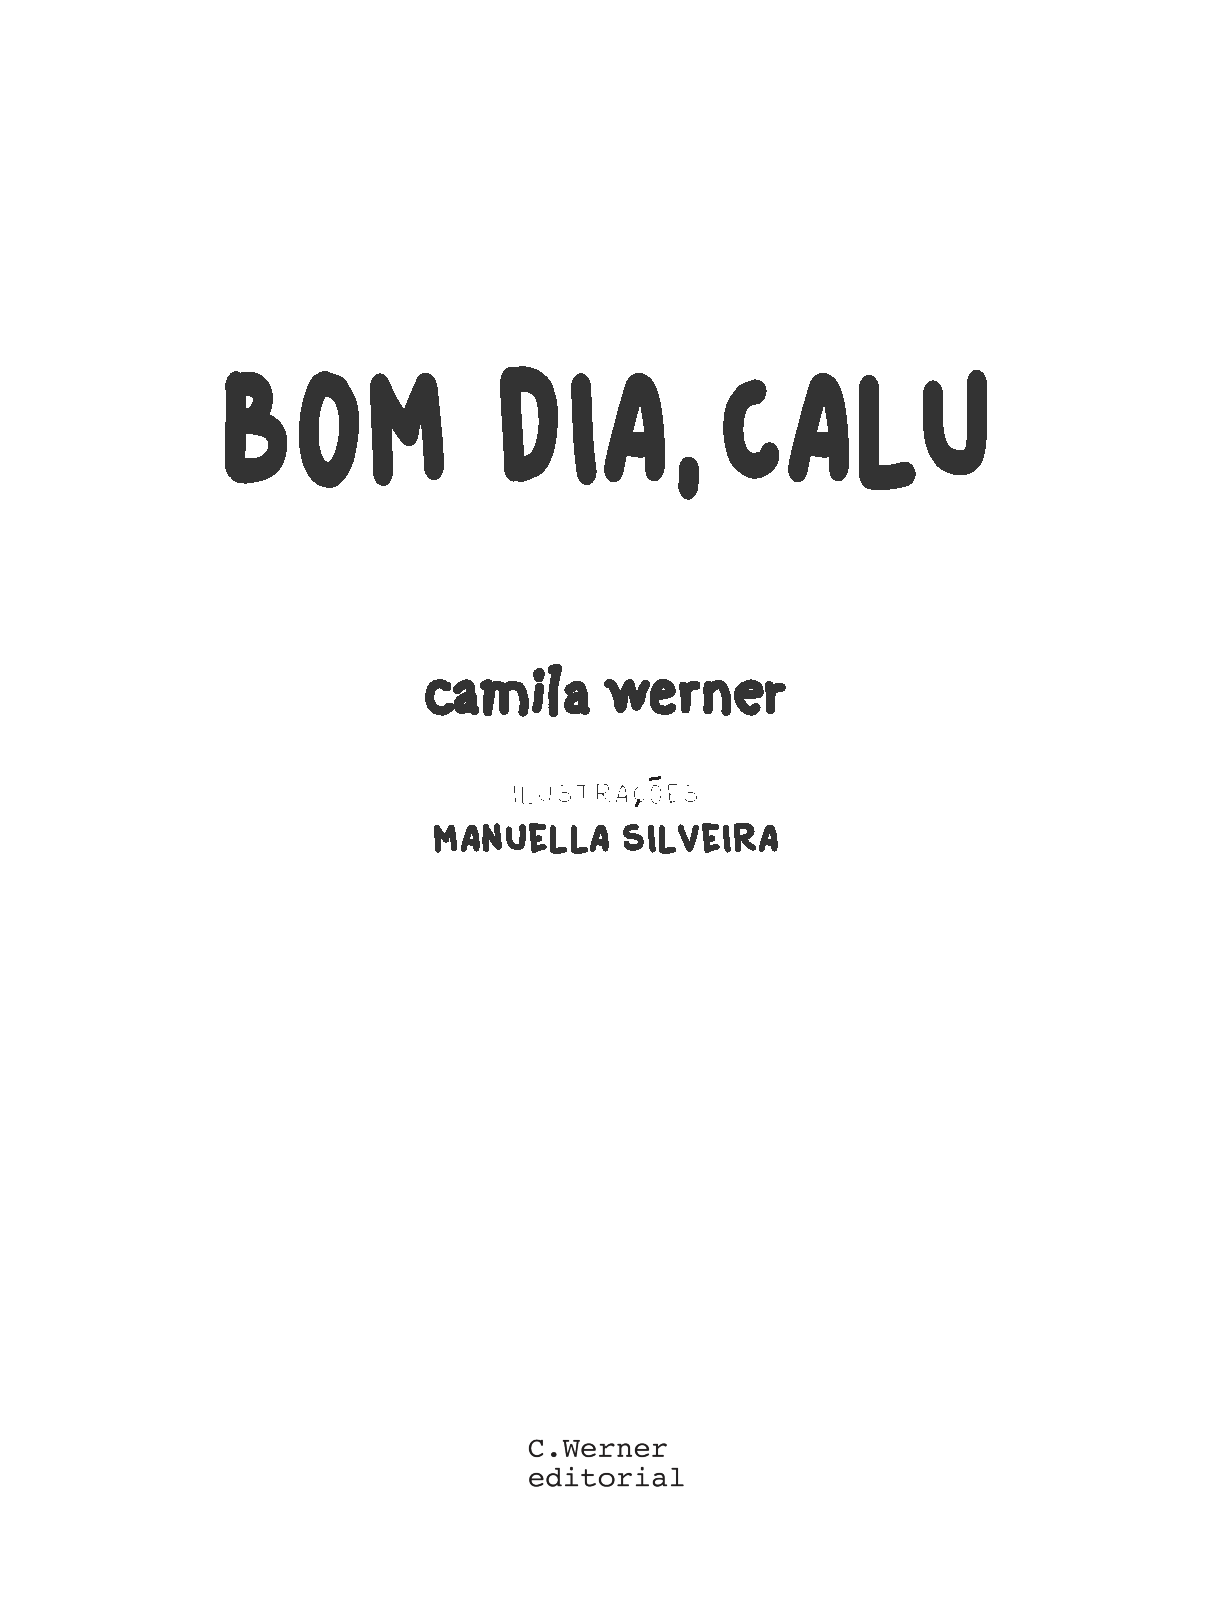
\includepdf[nup=2x2, 					% grid
			% offset=-15mm -5mm, 		% posição
			% scale=.8, 				% tamanho da página
            % delta=4mm 4mm, 			
            % frame,
            % pages={1-4}]{pdfs/PNLD2022-006_MIOLO.pdf}

\end{document}
